\documentclass[10pt,aps,onecolumn,superscriptaddress]{revtex4-2}

\usepackage[T1]{fontenc}
\usepackage[utf8]{inputenc}
\usepackage[english]{babel}

\usepackage{amsfonts,amsbsy,amssymb,amsmath,graphicx,float} 
\usepackage{color}
\usepackage{multirow}

\graphicspath{{figures/}}

\usepackage[linktoc=all,colorlinks=true,citecolor=blue,linkcolor=blue]{hyperref}

\bibliographystyle{apsrev4-2}

\renewcommand*\tocname{\large Contents}
\setcounter{tocdepth}{2} % + show subsections

% Commands for Mathematical Formulas
\newcommand{\mbf}[1]{\mathbf{#1}}
\newcommand{\pder}[2]{\dfrac{\partial{#1}}{\partial{#2}}}
\newcommand{\pderalt}[2]{\dfrac{\partial}{\partial{#2}}\left(#1\right)}
\newcommand{\pderalttwo}[3]{\dfrac{\partial^{2}}{\partial{#2}\partial{#3}}\left(#1\right)}
\newcommand{\pdertwo}[3]{\dfrac{\partial^{\,2} #1}{\partial{#2}\partial{#3}}}
\newcommand{\spdalt}[2]{\dfrac{\partial^{2}}{\partial{#2}^{2}}\left(#1\right)}
\newcommand{\spd}[2]{\dfrac{\partial^{\,2} #1}{\partial{#2}^{2}}}

\begin{document}

\maketitle



\section{Introduction}


In this section we continue the study of Collins et al. \cite{collins2011} by considering the phase space structures that govern different reaction pathways and we  then consider the influence of symmetry breaking, bifurcation, and energy on these phase space reaction pathways.

Consider thus the Hamiltonian:
\begin{equation}
H(x,y,p_x,p_y) = \frac{1}{2}\left(p_x^2 + p_y^2\right) + V(x,y)
\label{hamiltonian}
\end{equation}
where we have supposed for simplicity that the mass in each DoF is $m_x = m_y = 1$. The PES is defined as follows:
\begin{equation}
V(x,y) = x^4 - \alpha x^2 - \delta x + y^4 - y^2 + \beta x^2 y^2
\label{pes_model}
\end{equation}
and $\delta$ represents the asymmetry parameter in the double well potential of the $x$ DoF. The dynamics of the Hamiltonian in Eq. \eqref{hamiltonian} is described by Hamilton's equations of motion:
\begin{equation}
\begin{cases}
\dot{x} = \dfrac{\partial H}{\partial p_x} = p_x \\[.4cm]
\dot{y} = \dfrac{\partial H}{\partial p_y} = p_y \\[.4cm]
\dot{p}_x = -\dfrac{\partial H}{\partial x} = -\dfrac{\partial V}{\partial x} = -4 x^3 + 2 \alpha x + \delta - 2 \beta x y^2 \\[.4cm]
\dot{p}_y = -\dfrac{\partial H}{\partial y} = -\dfrac{\partial V}{\partial y} = -4 y^3 + 2 y - 2 \beta x^2 y
\end{cases}
\label{ham_eqs}
\end{equation}

	\begin{figure}[htbp]
		\begin{center}
		
			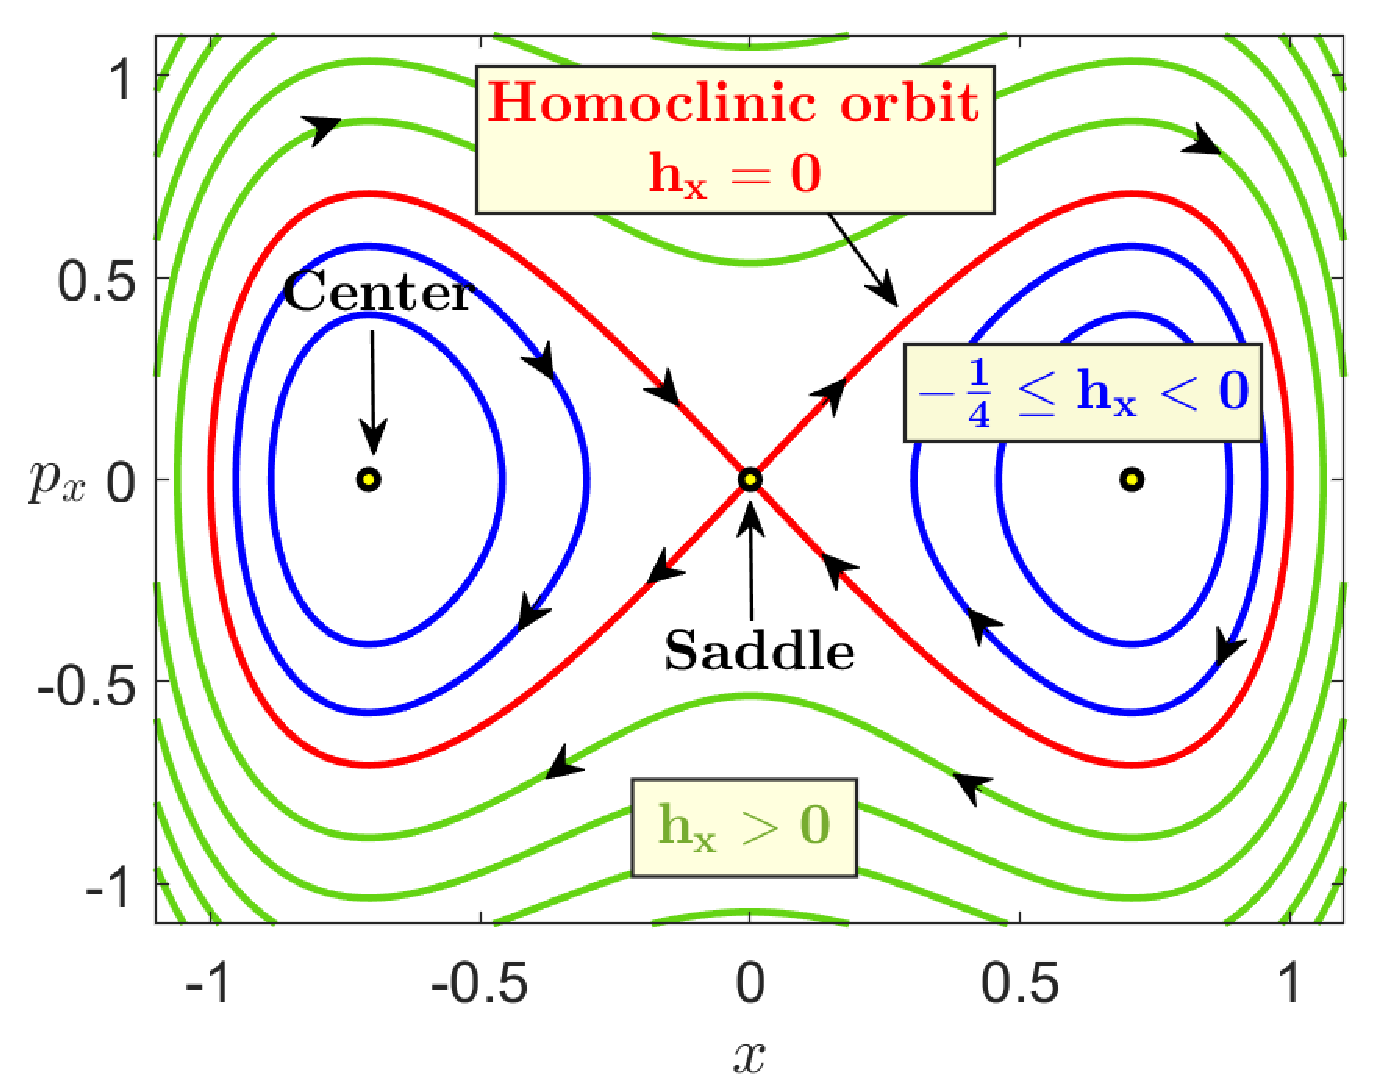
\includegraphics[scale=0.34]{phasePort_symm_1D_xDoF}
		\end{center}
		\caption{Depicts the phase portraits for the $x-p_x$  plane. We have marked with a magenta line the dividing surface $x = 0$ that separates the upper-left and upper-right wells of the PES.}
		\label{phasePort_1DoF_symm}
	\end{figure}

\bibliography{SNreac}
\end{document}
